\section{Examples of Algebraic Expressions}

Let's look at some basic algebraic expressions, describe them verbally, and evaluate them for some values of the variables.

\par

\begin{eg} Consider the algebraic expression
\[
(3x+1)^2-2.
\]
This expression only contains one variable, $x$. We can substitute values for $x$ and get values of the algebraic expression. For instance, if we evaluate it at $x=2$ we get
\[
(3\cdot 2+1)^2 -2 = 7^2-2 = 47.
\]
If we evaluate this expression at $x=-2$ we have
\[
(3\cdot(-2) +1)^2 -2 = (-5)^2 -2 = 23,
\]
Evaluating algebraic expressions isn't that hard provided you keep track of your order of operations. A more difficult, but very much related skill is to read an algebraic expression and verbally express what is being done to the variable(s) in the correct order. In this expression we start with the value of $x$ and
\begin{enumerate}
\item[\bf S1:] multiply $x$ by three,
\item[\bf S2:] add one to the result of {\bf S1}
\item[\bf S3:] square the result of {\bf S2}, and finally
\item[\bf S4:] subtract two from the result of {\bf S3}.  
\end{enumerate}
\qed
\end{eg}

This idea of verbally describing algebraic expressions and understanding the steps that they represent is important for seeing algebraic expressions as something other than just a bunch of random symbols on a page. 
\begin{center}
Algebraic Expressions Describe Processes Performed on Variables 
\begin{tabular}{|p{1.5in} c p{2.5in} |}
\hline\hline \it{Algebraic Expression} & $\longrightarrow$ & \it{A symbolic representation of a sequence  of arithmetic operations performed in a specific order on general numbers (variables).}\\
\hline
\end{tabular}
\end{center}

\begin{question} Write an algebraic expression that represents the following process applied to $x$:
\begin{enumerate}
\item[\bf S1:] Add one to $x$,
\item[\bf S2:] square the result of {\bf S1}
\item[\bf S3:] subtract two from the result of {\bf S2}, and finally
\item[\bf S4:] multiply the result of {\bf S3} by $5$.  
\end{enumerate}
Evaluate the expression you get at $x=2$, $x=-2$, and $x=0$.
\end{question}

\par
We will often abbreviate the result of a step {\bf Sn} by just writing {\bf Sn}.  For example, we could just write "multiply {\bf S3} by $5$" for the last step above.  
\par

\begin{eg} \label{E:recip}  Suppose we want to understand the expression $\frac{2}{x+1}$.  One way to describe this process is
\begin{enumerate}
\item[\bf S1:] Add $1$ to $x$, 
\item[\bf S2:] divide $2$ by {\bf S1}. 
\end{enumerate}
Note that we need to be careful in describing {\bf S2}:  we need to specify which quantity is divided by which here.  
We may want to think of this as a process which is being done primarily to $x$, and break it down as $2 \cdot \frac{1}{x+1}$.  Then we could describe the expression by the following: 
\begin{enumerate}
\item[\bf S1:] Add $1$ to  $x$
\item[\bf S2:] Take the reciprocal of {\bf S1}
\item[\bf S3:] multiply the result of {\bf S2} by $2$.  
\end{enumerate}
\end{eg}
\par
Sometimes a variable can appear more than once in an expression, which may make describing it as a single procedure more difficult. This difficulty is dealt with by thinking of a combination of procedures using order of operations.

\par

\begin{eg} Verbally describe the expression
\[
4s^2 + 2\sqrt{s+1}.
\]
If we were evaluating this at a specific value of $s$, we would perform the addition last. For this reason, we take each part that will be added together and describe them separately first. For the first term (a \it{term }\normalfont is a part of an algebraic expression being added to other parts):
\begin{enumerate}
\item[\bf S1:] Square $s$, then
\item[\bf S2:] multiply {\bf S1} by four.
\end{enumerate}
Then we pick up with the second term:
\begin{enumerate}
\item[\bf S3:] Add one to $s$,
\item[\bf S4:] take the square root of {\bf S3}, and
\item[\bf S5:] multiply {\bf S4} by two.
\end{enumerate}
The last step is the last thing according to our order of operations:

\begin{enumerate}
\item[\bf S6:] Add the result of {\bf S2} to the result of steps {\bf S5}.  \qed
\end{enumerate}
\end{eg}

\begin{question} List the steps being performed on $x$, in order, for each of the following algebraic expressions:
\begin{enumerate}
\item $\frac{6}{2+x}$
\item $2(x+1)^2 -5$
\item $3(x+2)-5(x-7)$
\item $\frac{3}{x} - 4x^2 -1$
\item $\frac{1}{x-a}+\frac{3}{\sqrt{x+b}}$
\end{enumerate}
\end{question}

Let's finish this section with examples of algebraic expressions that you might come across in another class or the real world.

\par

\begin{eg} An algebraic expression commonly encountered in a first year physics course gives the height $h$ of a projectile, in meters, above the ground $t$ seconds after it has been launched. This expression has parameters for initial height and initial upward velocity. The expression is
\[
h = -4.9t^2+v_0 t + h_0,
\]
where $v_0$ is the initial upward velocity in m/s and $h_0$ is the initial height in meters. For instance, if we knew the initial height was $40$ meters and the initial velocity was $0$ m/s (if the object was dropped, not thrown), then we would have
\[
h = -4.9t^2 + 40.
\]
\qed  
  \end{eg}
\par 

\begin{question} Using the expression above, with $h_0 = 40$ and $v_0 = 0$, for the height, answer the following questions to the best of your ability (you may need a calculator).
\begin{enumerate}
\item[a.] How high is the object after $2$ seconds? $3$ seconds?
\item[b.] When does the object hit the ground?
\item[c.] Is the object ever $50$ meters above the ground? Justify your answer in practical terms and algebraically, if possible.
\end{enumerate}
\end{question}

\par 

\begin{eg} The following table gives the men's world record times for running events as of Summer 2017, as well as the average speeds in m/s.\\
\begin{center}
\begin{tabular}{| c | c | c |}
\hline $d=$\ Distance (m) & $T=$\ time (s) & $S=$\ speed (m/s)\\
\hline\hline 100  & 9.58 & 10.44\\
\hline 200 & 19.19 & 10.42\\
\hline 400 & 43.03 & 9.3\\
\hline 800 & 100.91 & 7.93\\
\hline 1500 & 206 & 7.28\\
\hline 5000 & 757.35 & 6.6\\
\hline
\end{tabular}
\end{center}
Using techniques from statistics or linear algebra (data fitting), it is possible to give an algebraic expression involving the distance $d$ that approximately tells you the record time $T$. The expression one finds this way is
\[
T = .06640993d^{1.09689}.
\]
Since speed is distance divided by time, we can then formulate an expression for the speed $S$ in terms of the distance $d$:
\[
S = \frac{d}{T}  = \frac{d}{.06640993 d^{1.09689}} = \frac{15.05798907}{d^{.09689}}.
\]
\qed
\end{eg}

\begin{question} Use the expressions in the last example to answer the following questions.  
\begin{enumerate} 
\item[a.] The expressions given above only give approximations. After all, if we could find record times with a formula we wouldn't need to have races. Use a calculator to evaluate the expression given for $T$, for each distance, and see how well it matches the data.
\item[b.] What does the expression for $T$ say the record time for $10000$ meters should be? Is it accurate? (Use the internet to check.)
\item[c.] Two versions of the expression for $S$ are shown. Use the rules for fractions and exponents from Chapter 1 to explain why these two versions are really the same.
\item[d.] In the expression for $S$, what happens to $S$ as $d$ gets very large (see Question 1.5a in Chapter 1)? Does this make practical sense?
\end{enumerate}  
\end{question}
 

\section{Equivalent Algebraic Expressions}

Two algebraic expressions are called \it{equivalent} \normalfont if they yield the same output no matter what is substituted into them. Thinking of algebraic expressions procedurally, we have the following characterization of equivalent algebraic expressions:

\begin{center}
Equivalent Expressions as Different Processes with the Same Result
\begin{tabular}{|p{2.5in} c p{2.5in} |}
\hline\hline \it{Equivalent Algebraic Expressions} & $\rightarrow$ & \it{Equivalent algebraic expressions are symbolic representations of different processes performed on the variables that always give the same end result.}\\
\hline
\end{tabular}
\end{center}

\par

People who are good at algebra often speak of manipulating/simplifying algebraic expressions and putting expressions into different forms. What they are talking about is replacing an expression with an equivalent expression. The reason for manipulating expressions is that sometimes one version of an expression makes it easier to see a solution to a problem. For instance, the expression used to find the temperature in $^{\circ}$C given the temperature in $^{\circ}$F is
\[
C = \frac{5}{9}F - \frac{160}{9},
\]
where $F$ is the temperature in $^{\circ}$F and $C$ is the temperature in $^{\circ}$C. Suppose we want to know what temperature in $^{\circ}$F corresponds to $O^{\circ}$C. Even if you already know the answer is $32^{\circ}$F, the given expression does not make it obvious. However, the given expression is equivalent to the following:
\[
C = \frac{5}{9}(F - 32).
\]
Now the solution is more clear; if we substitute $F=32$ into the expression for $C$ in terms of $F$, we get $\frac{5}{9}(32-32) = 0$. 
\par
Why are these two expressions equivalent? The answer here comes from the arithmetic rule known as the distributive law (to be discussed more later). We can take the second expression and distribute the $\frac{5}{9}$ as follows:
\[
\frac{5}{9}(F-32)  = \frac{5}{9}F - \frac{5}{9}\cdot 32 = \frac{5}{9}F-\frac{160}{9}.
\]

Another example of equivalent expressions is give by Example \ref{E:recip}.    In this case, we used the fact that the expression $\frac{2}{x+1}$ is equivalent to $2 \cdot \frac{1}{x+1}$.  

Fundamentally, since algebraic expressions are built using the operations of arithmetic, equivalence of algebraic expressions is determined by using rules of arithmetic. We will discuss the most commonly used ways of manipulating expressions into equivalent ones in the remainder of this section. However, we will first discuss how to tell if two expressions are inequivalent.

\subsection{Inequivalent Expressions}

Two expressions are not equivalent if there are some values of the variables in the expression that yield different numbers when you substitute. So, if you plug the same number into two expressions and get different results, then the two expressions are inequivalent (assuming you did the arithmetic correctly). With practice, you'll get good at being able to detect inequivalent expressions without even needing to substitute anything. For now, we'll look at some important examples that sometimes trip people up.

\par

\begin{eg}
The two expressions $(x+y)^2$ and $x^2 + y^2$ are \underline{not}\normalfont\ equivalent. One may detect this by noting the order in which operations are performed on $x$ and $y$. In one expression you add the two variables, then square. In the other, you square each variable, then add. Based one our experience with order of operations (order matters), we think these may not be equivalent. It turns out that if you pick any two numbers for $x$ and $y$, as long as neither is zero, these two expressions will evaluate to different numbers. For instance, if we substitute $x=1$ and $y=2$, then the first expression gives 
\[
(1+2)^2 = 3^2 =9,
\]
whereas the second expression gives
\[
1^2+2^2 = 1+4 = 5.
\]
It is also possible to see that these two expressions are inequivalent by giving the geometric representations. We begin by thinking of $x$ and $y$ as lengths. Then $(x+y)^2$ is the area of a square whose side length is $x+y$, while $x^2+y^2$ is the sum of areas of squares that fit inside the square of side length $x+y$ as in the following diagram:

\vspace{.2in}
\begin{figure}[h]
\centering
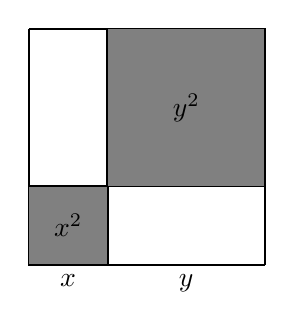
\begin{tikzpicture}
\draw[thick] [-] (0,0) -- (1,0);
\draw[thick] [-] (1,0) -- (3,0);
\draw[thick] [-] (0,0) -- (0,1);
\draw[thick] [-] (0,1) -- (0,3);
\draw[thick] [-] (1,0) -- (1,3);
\draw[thick] [-] (0,1) -- (3,1);
\draw[thick] [-] (0,3) -- (3,3);
\draw[thick] [-] (3,0) -- (3,3);
\draw [fill=gray] (0,0) rectangle (1,1);
\draw [fill=gray] (1,1) rectangle (3,3);
\node[align=center,below] at (.5,0){$x$};
\node[align=center,below] at (2,0){$y$};
\node[align=center] at (.5,.5){$x^2$};
\node[align=center] at (2,2){$y^2$};
\end{tikzpicture}
\end{figure}



In this figure we see that the total shaded area is $x^2+y^2$ while the area of the entire square is $(x+y)^2$. If you note that the unshaded portions of the square each have area $xy$, we can see that $(x+y)^2$ \underline{is}\normalfont\ equivalent to $x^2+2xy+y^2$. We will see this more symbolically in the section on distributing, expanding, and factoring. \qed
\end{eg}

\par

\begin{question} Explain why $\sqrt{a^2 + b^2}$ is not equivalent to $a+b$. Do this both by plugging in numbers and by either referring to the last example, or using the Pythagorean Theorem to explain the inequivalence geometrically.
\end{question}

\par

\begin{question} Use volumes to give a geometric explanation of why $(x+y)^3$ is equivalent to $x^3+3x^2y+3xy^2+y^3$, but is not equivalent to $x^3+y^3$.
\end{question}

\par 

\begin{eg} $\frac{1}{x}+\frac{1}{3}$ is \underline{not}\normalfont\ equivalent to $\frac{2}{x+3}$. A simple, but perhaps not helpful, reason is because that's not how you add fractions. Let's make sure we really see that this is not how you add fractions. First substitute $x=1$. Then the first expression evaluates to
\[
\frac{1}{1} + \frac{1}{3}=1+\frac{1}{3},
\]  
while the second evaluates to
\[
\frac{2}{4} = \frac{1}{2}.
\]
Even if you forget how to add fractions you can tell these are not equal. The first one is larger than one and the second is smaller than one.
\qed
\end{eg}
\par 

{\bf Remark:} It is important to note that for two expressions to be equivalent, they must evaluate to the same number for \underline{all}\normalfont\ values of the variables, not just some. For instance, in the example with squares, if $x=0$ the two expressions do evaluate to the same thing. However, this does not make the expressions equivalent.\qed  

\subsection{Reordering and Regrouping}

Sometimes the order in which operations are performed in an algebraic expression doesn't affect the result. Specifically, if the expression only involves addition, order of operations doesn't tell you which one to do first because it doesn't matter. Likewise for multiplication. Specifically, we have the following rules for addition and multiplication:

\begin{tcolorbox}
{\bf Commutative and Associative Laws for Addition and Multiplication}
\begin{itemize}
\item $a+b = b+a$ (addition is commutative)
\item $ab=ba$ (multiplication is commutative)
\item $a+(b+c) = (a+b)+c$ (addition is associative)
\item $a(bc)=(ab)c$ (multiplication is associative)
\end{itemize}
\end{tcolorbox}

In Chapter 1 you were asked to explain the commutativity of addition geometrically using lengths on the number line (Question 1). To explain the commutativity of multiplication, we think of $a$ and $b$ as lengths of the sides of a rectangle. Using the fact that the area of a rectangle is given by
\[
\mbox{Area} = \mbox{base}\times\mbox{height},
\]
we can arrange our rectangle with $a$ on the bottom and $b$ on the side to get the area to be $ab$. If we simply rotate the rectangle $90$ degrees, the are is then seen as $ba$. Since rotation doesn't change the area, we must have $ab = ba$.

\begin{figure}[h]
\centering
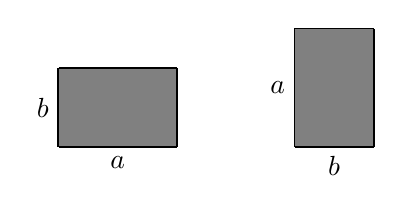
\begin{tikzpicture}
\draw[thick] [-] (0,0) -- (1.5,0);
\draw[thick] [-] (0,0) -- (0,1);
\draw[thick] [-] (0,1) -- (1.5,1);
\draw[thick] [-] (1.5,1) -- (1.5,0);
\draw[thick] [-] (3,0) -- (4,0);
\draw[thick] [-] (3,0) -- (3,1.5);
\draw[thick] [-] (3,1.5) -- (4,1.5);
\draw[thick] [-] (4,1.5) -- (4,0);
\draw [fill=gray] (0,0) rectangle (1.5,1);
\draw [fill=gray] (3,0) rectangle (4,1.5);
\node[align=center,below] at (.75,0){$a$};
\node[align=center,left] at (0,.5){$b$};
\node[align=center,below] at (3.5,0){$b$};
\node[align=center,left] at (3,.75){$a$};
\end{tikzpicture}
\caption{These rectangles have the same area, so $ab=ba$}
\end{figure}


\begin{question} Now we would like geometric explanations of the associative laws.
\begin{enumerate}
\item[a.] Explain the associative law for addition using lengths on the number line.
\item[b.] Explain the associative law for multiplication using the fact that the volume of a rectangular prism is the area of its base multiplied by its height (similar to our explanation of the commutative law for multiplication).
\end{enumerate}
\end{question}

These rules are most useful in simplifying complex expressions that involve many terms being added together or multiplied.

\begin{eg}
 Suppose you have two cans, both are $5$ inches tall, but one has a diameter that it three times that of the other one. Let $d$ denote the diameter of the smaller can, in inches. Suppose we would like to find a simplified expression for the total volume of the two cans in terms of $d$. First we note the formula for the volume of a cylinder: $V=\pi r^2h$, where $r$ is the radius and $h$ is the height. Since both cans have a height of $5$ inches, we substitute $h = 5$. Since $r= \frac{d}{2}$, the volume of the first can is then given by $\pi\cdot\left(\frac{d}{2}\right)^2\cdot 5$. Using associativity and commutativity, this simplifies to
\[
\mbox{volume of smaller can} = \frac{5}{4}\pi d^2\ \mbox{in}^3.
\]
Since the diameter of the larger can is three times that of the smaller can, its radius is $\frac{3d}{2}$, which makes its volume
\[
\mbox{volume of larger can} = \pi\cdot\left(\frac{3d}{2}\right)^2\cdot 5 = \frac{45}{4} \pi d^2\ \mbox{in}^3.
\]
Adding them together we have
\[
\mbox{Total Volume} = \frac{5}{4}\pi d^2 + \frac{45}{4}\pi d^2 = \frac{25}{2}\pi d^2\ \mbox{in}^3.
\]
\qed
\end{eg}

In the last step of the last example we performed an important type of regrouping known as \it{combining like terms}\normalfont. This is when all the terms with the same algebraic type (same exponents on a variable for example) are combined into a single term by adding together the constants by which they are multiplied. It is important to note that terms can only be combined when the only difference between them is a constant multiplier. For instance,
\[
3x^2 + 4\sqrt{x} + 5x^2 - \sqrt{9x} = 8x^2+4\sqrt{x}-3\sqrt{x} = 8x^2+\sqrt{x}.
\]
The remaining terms cannot be combined further because one has an exponent of $2$ while the other has an exponent of $\frac{1}{2}$.

\par

\begin{eg} Let's see another reason unlike terms can't be combined. Consider the expression $4x^3+ 6x$. To make it more meaningful, we may think of $x$ as a length with units of meters. Then $x^3$ represents a volume in cubic meters.  Because of dimensional considerations, $x$ and $x^3$ cannot be combined in a meaningful way. In order for this expression to make any practical sense when $x$ is in meters, the $6$ needs to be in square meters. However, then the $4$ is dimensionless, while the $6$ represents an area.  We cannot add the $4$ and the $6$, since they represent different units.   So thinking of $4x^3 + 6x$ as representing some geometric quantity shows that it cannot be simplified any further.\qed

\end{eg}

\begin{question} Give a collection of objects (geometric shapes, not necessarily real-world objects) that would have a volume represented by $4x^3 + 6x$?
\end{question}

\begin{question} Decide if the following attempts to combine like terms are correct. If a mistake was made, say what it was and correct it.
\begin{enumerate}
\item[a.] $4xy+7y^2x + 3x^2y +2yx = 6xy + 10x^3y^3$
\item[b.] $(2x^2+1) + (3x+7) + (x^2-8x) = 3x^2-5x+8$
\end{enumerate} 
\end{question}  

\subsection{Distributing, Expanding, and Factoring}

One of the most important rules in constructing equivalent algebraic expressions is the Distributive Law.

\begin{tcolorbox}
{\bf The Distributive Law}
For any $a$, $b$, and $c$
\[
a(b+c) = ab+ac.
\] 
\end{tcolorbox}

This fact asserts that you can
\begin{itemize}
\item add two lengths, $b$ and $c$, on the line together, then expand/compress by a factor of $a$, or
\item expand/contract each of $b$ and $c$ by a factor of $a$, then add the results together. 
\end{itemize}
The end result is the same in either case. Many seemingly complex algebraic manipulations boil down to using the distributive law several times and collecting like terms; it's just that $a$, $b$, and $c$ may be some sort of algebraic expressions.

\par 

\begin{eg} Let's find the expanded form of $(x+y)^2$ using the distributive law. 
\begin{eqnarray*}
(x+y)^2 & = & (x+y)(x+y)\\
 & = & (x+y)x + (x+y)y  \phantom{www} \mbox{the distributive law}\\
 & = & (x^2+xy) + (xy+y^2) \phantom{wn} \mbox{more distributive law}\\
 & = & x^2+2xy+y^2 \phantom{wwwwwwi} \mbox{combining like terms}
\end{eqnarray*}\qed
\end{eg}
\par 

\begin{question} Describe what each term in the second and third lines of the manipulation given above represents geometrically as areas, as in the example in the last section showing $(x+y)^2 = x^2+2xy+y^2$.
\end{question}

\begin{eg} Subtraction of quantities in parentheses is often simplified using the distributive law and remembering that subtraction is really just addition of $-1$ times the given quantity. For instance, suppose we want to simplify the expression
\[
3x^2 - (4x+2x^2)
\]
First, re-write it with addition and $-1$ multiplying the piece in parentheses, then apply the distributive law:
\begin{eqnarray*}
3x^2 - (4x+2x^2) & = & 3x^2 + (-1)(4x+2x^2)\\
\ & = & 3x^2+((-1)4x+(-1)2x^2)\\
\ & = & 3x^2-4x-2x^2\\
\ & = & x^2-4x.
\end{eqnarray*}
With practice, you probably won't need to write this many steps down. This process is often referred to as ``distributing a minus sign''.\qed
\end{eg}

Now is probably a good time to just get a little practice expanding/distributing and collecting like terms. Just remember the distributive law and you'll see it's not that hard.

\par 

\begin{question} Expand (write as an equivalent expression without parentheses) each of the following expressions and collect like terms:
\begin{enumerate}
\item[a.] $3ab(2a-5b)$
\item[b.] $(2x+1)(3x-4)$
\item[c.] $3x^2(1-x)^3$
\item[d.] $2x-\frac{1}{3}x(5-3x-2x^2)$
\end{enumerate}
\end{question}

\par 

Now we will go backward from expanding/distributing. This process is known as factoring. When we expand an expression, we write it as an equivalent expression that is a sum of simple terms that each only involve multiplication and/or division. To \it{factor}\ \normalfont an expression means to write it as a product of simple terms. For example, earlier in this chapter we had two expressions for the temperature in $^{\circ}$C in terms of the temperature in $^{\circ}$F. The expression $C = \frac{5}{9}F - \frac{160}{9}$ is in expanded form, while $C = \frac{5}{9}(F-32)$ is in factored form. Factored forms of expressions are often useful for solving equations as we'll see in the next chapter. Factoring isn't something that can be done in all cases by a single procedure; the following are just a few examples of common factoring methods.

\par 

\begin{eg} When each term of an expression is divisible by some common factor one can ``un-distribute'' that factor. For instance, if we are given the expression
\[
12xy+6y^2+3y^3,
\]
we can see that each term contains $y$ and $3$ as a factor. This means we can factor $3y$ out of the expression to get the equivalent expression
\[
3y(4x+2y+y^2).
\]
Note that you can check your answer by applying the distributive law. An interpretation of pulling out a common factor like this is that each term is being stretched/compressed by the same amount, hence we can think of this as a single entity being stretched/compressed, which may be simpler.\qed
\end{eg}
\par

\begin{eg} Expressions of the form $ax^2+bx+c$, where $a$, $b$, and $c$ are constants are known as {\bf quadratic} expressions in the variable $x$. Factoring such expressions is a very common and useful algebraic task. It is possible to give a procedure for factoring quadratics, but right now it is best to proceed with examples and practice. For instance, consider the expression
\[
12x^2+5x-2.
\]
We wish to re-write this expression in the form
\[
(rx+p)(sx+q).
\]
We note that
\begin{itemize}
\item $rs$ must equal $12$, 
\item $pq$ must equal $-2$, and
\item $rq + ps$ must equal $5$. 
\end{itemize}
Some trial and error leads us to 
\[
(3x+2)(4x-1),
\]
which we may check by expanding. \qed
\end{eg}



\begin{eg} Any expression of the form $a^2-b^2$ may be factored as $(a+b)(a-b)$ ($a$ and $b$ may represent more complicated expressions in this). One may check this using the distributive law. To see how this factorization works geometrically, consider the following figure with $b$ being thought of as a number smaller than $a$.\\
\vspace{.2in}
\begin{figure}[h]
\centering
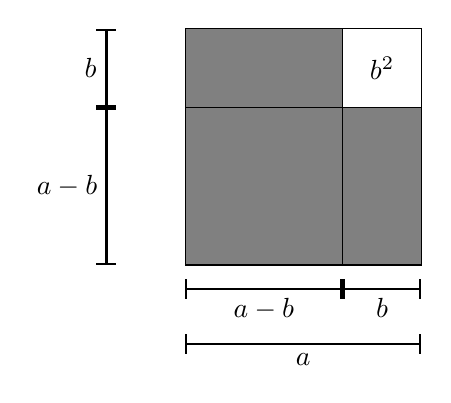
\begin{tikzpicture}
\draw[thick] [|-|] (-1,0) -- (-1,2);
\draw[thick] [|-|] (-1,2) -- (-1,3);
\draw[thick] [|-|] (0,-1) -- (3,-1);
\draw[thick] [|-|] (0,-.3) -- (2,-.3);
\draw[thick] [|-|] (2,-.3) -- (3,-.3);
\draw (2,2) rectangle (3,3);
\draw [fill=gray] (0,2) rectangle (2,3);
\draw [fill=gray] (0,0) rectangle (2,2);
\draw [fill=gray] (2,0) rectangle (3,2);
\node[align=center,below] at (1.5,-1){$a$};
\node[align=center,below] at (1,-.3){$a-b$};
\node[align=center] at (-1.5,1){$a-b$};
\node[align=center] at (-1.2,2.5){$b$};
\node[align=center,below] at (2.5,-.3){$b$};
\node[align=center] at (2.5,2.5){$b^2$};
\end{tikzpicture}
\end{figure}

In this figure the entire square has an area of $a^2$ units and the gray shaded area has an area of $a^2-b^2$ units. Each of the smaller shaded rectangles has area $b(a-b)$ and the lower right shaded square has an area of $(a-b)(a-b)$. Hence the total shaded area is
\[
a^2-b^2 = (a-b)(a-b) + 2b(a-b).
\]
Now each term has a common factor of $(a-b)$, hence we may factor it off and simplify by collecting like terms:
\begin{eqnarray*}
a^2-b^2 & = & (a-b)(a-b) + 2b(a-b)\\
\ & = & (a-b)(a-b+2b)\\
\ & = & (a-b)(a+b).
\end{eqnarray*}


One may also see this factorization geometrically by taking the shaded rectangle on top and moving it to the left hand side of the diagram.

\vspace{.2in}
\begin{figure}[h]
\centering
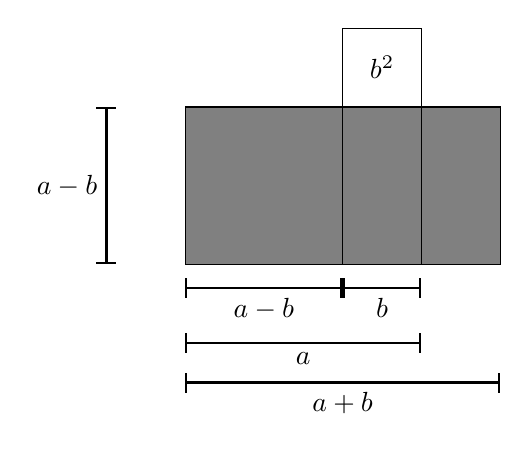
\begin{tikzpicture}
\draw[thick] [|-|] (-1,0) -- (-1,2);
\draw[thick] [|-|] (0,-1) -- (3,-1);
\draw[thick] [|-|] (0,-.3) -- (2,-.3);
\draw[thick] [|-|] (2,-.3) -- (3,-.3);
\draw[thick] [|-|] (0,-1.5) -- (4,-1.5);
\draw (2,2) rectangle (3,3);
\draw [fill=gray] (3,0) rectangle (4,2);
\draw [fill=gray] (0,0) rectangle (2,2);
\draw [fill=gray] (2,0) rectangle (3,2);
\node[align=center,below] at (1.5,-1){$a$};
\node[align=center,below] at (1,-.3){$a-b$};
\node[align=center] at (-1.5,1){$a-b$};
\node[align=center,below] at (2.5,-.3){$b$};
\node[align=center] at (2.5,2.5){$b^2$};
\node[align=center,below] at (2,-1.5){$a+b$};
\end{tikzpicture}
\end{figure}

Now we have a single shaded rectangle whose height is $a-b$ and whose width is $a+b$, hence the total area is $(a-b)(a+b)$.\qed

\end{eg}

\begin{question} Factor each of the following expressions as completely as possible.
\begin{enumerate}
\item[a.] $x^2+5x+6$
\item[b.] $x^4-25x^2y^2$
\item[c.] $4x^2+19x+12$
\item[d.] $y^2-y^4$
\item[e.] $2x^3-16x^2+32x$
\item[f.] $z^4+z^2-2$
\end{enumerate}
\end{question}

\begin{question} Think of $x$, $y$, and $1$ as positive lengths to use areas of rectangles to explain why
\[
6xy + 2y+6x+2 = (3x+1)(2y+2).
\]
\end{question}
 